Figure \ref{fig:img42_src} shows  Image4\_2 which has to be restored. This image  compared to the original  (Figure \ref{fig:orignal}) has some both horizontal and vertical stripes.   Based on the frequency spectrum of this image, it can be seen that some frequency component exist around the center frequency creating this effect. The purpose of this restoration will be to reduce the effect of these component, and reconstruct it so it resembles Figure \ref{fig:orignal}

\begin{figure}[H]
    \centering
    \begin{subfigure}[b]{0.23\textwidth}
        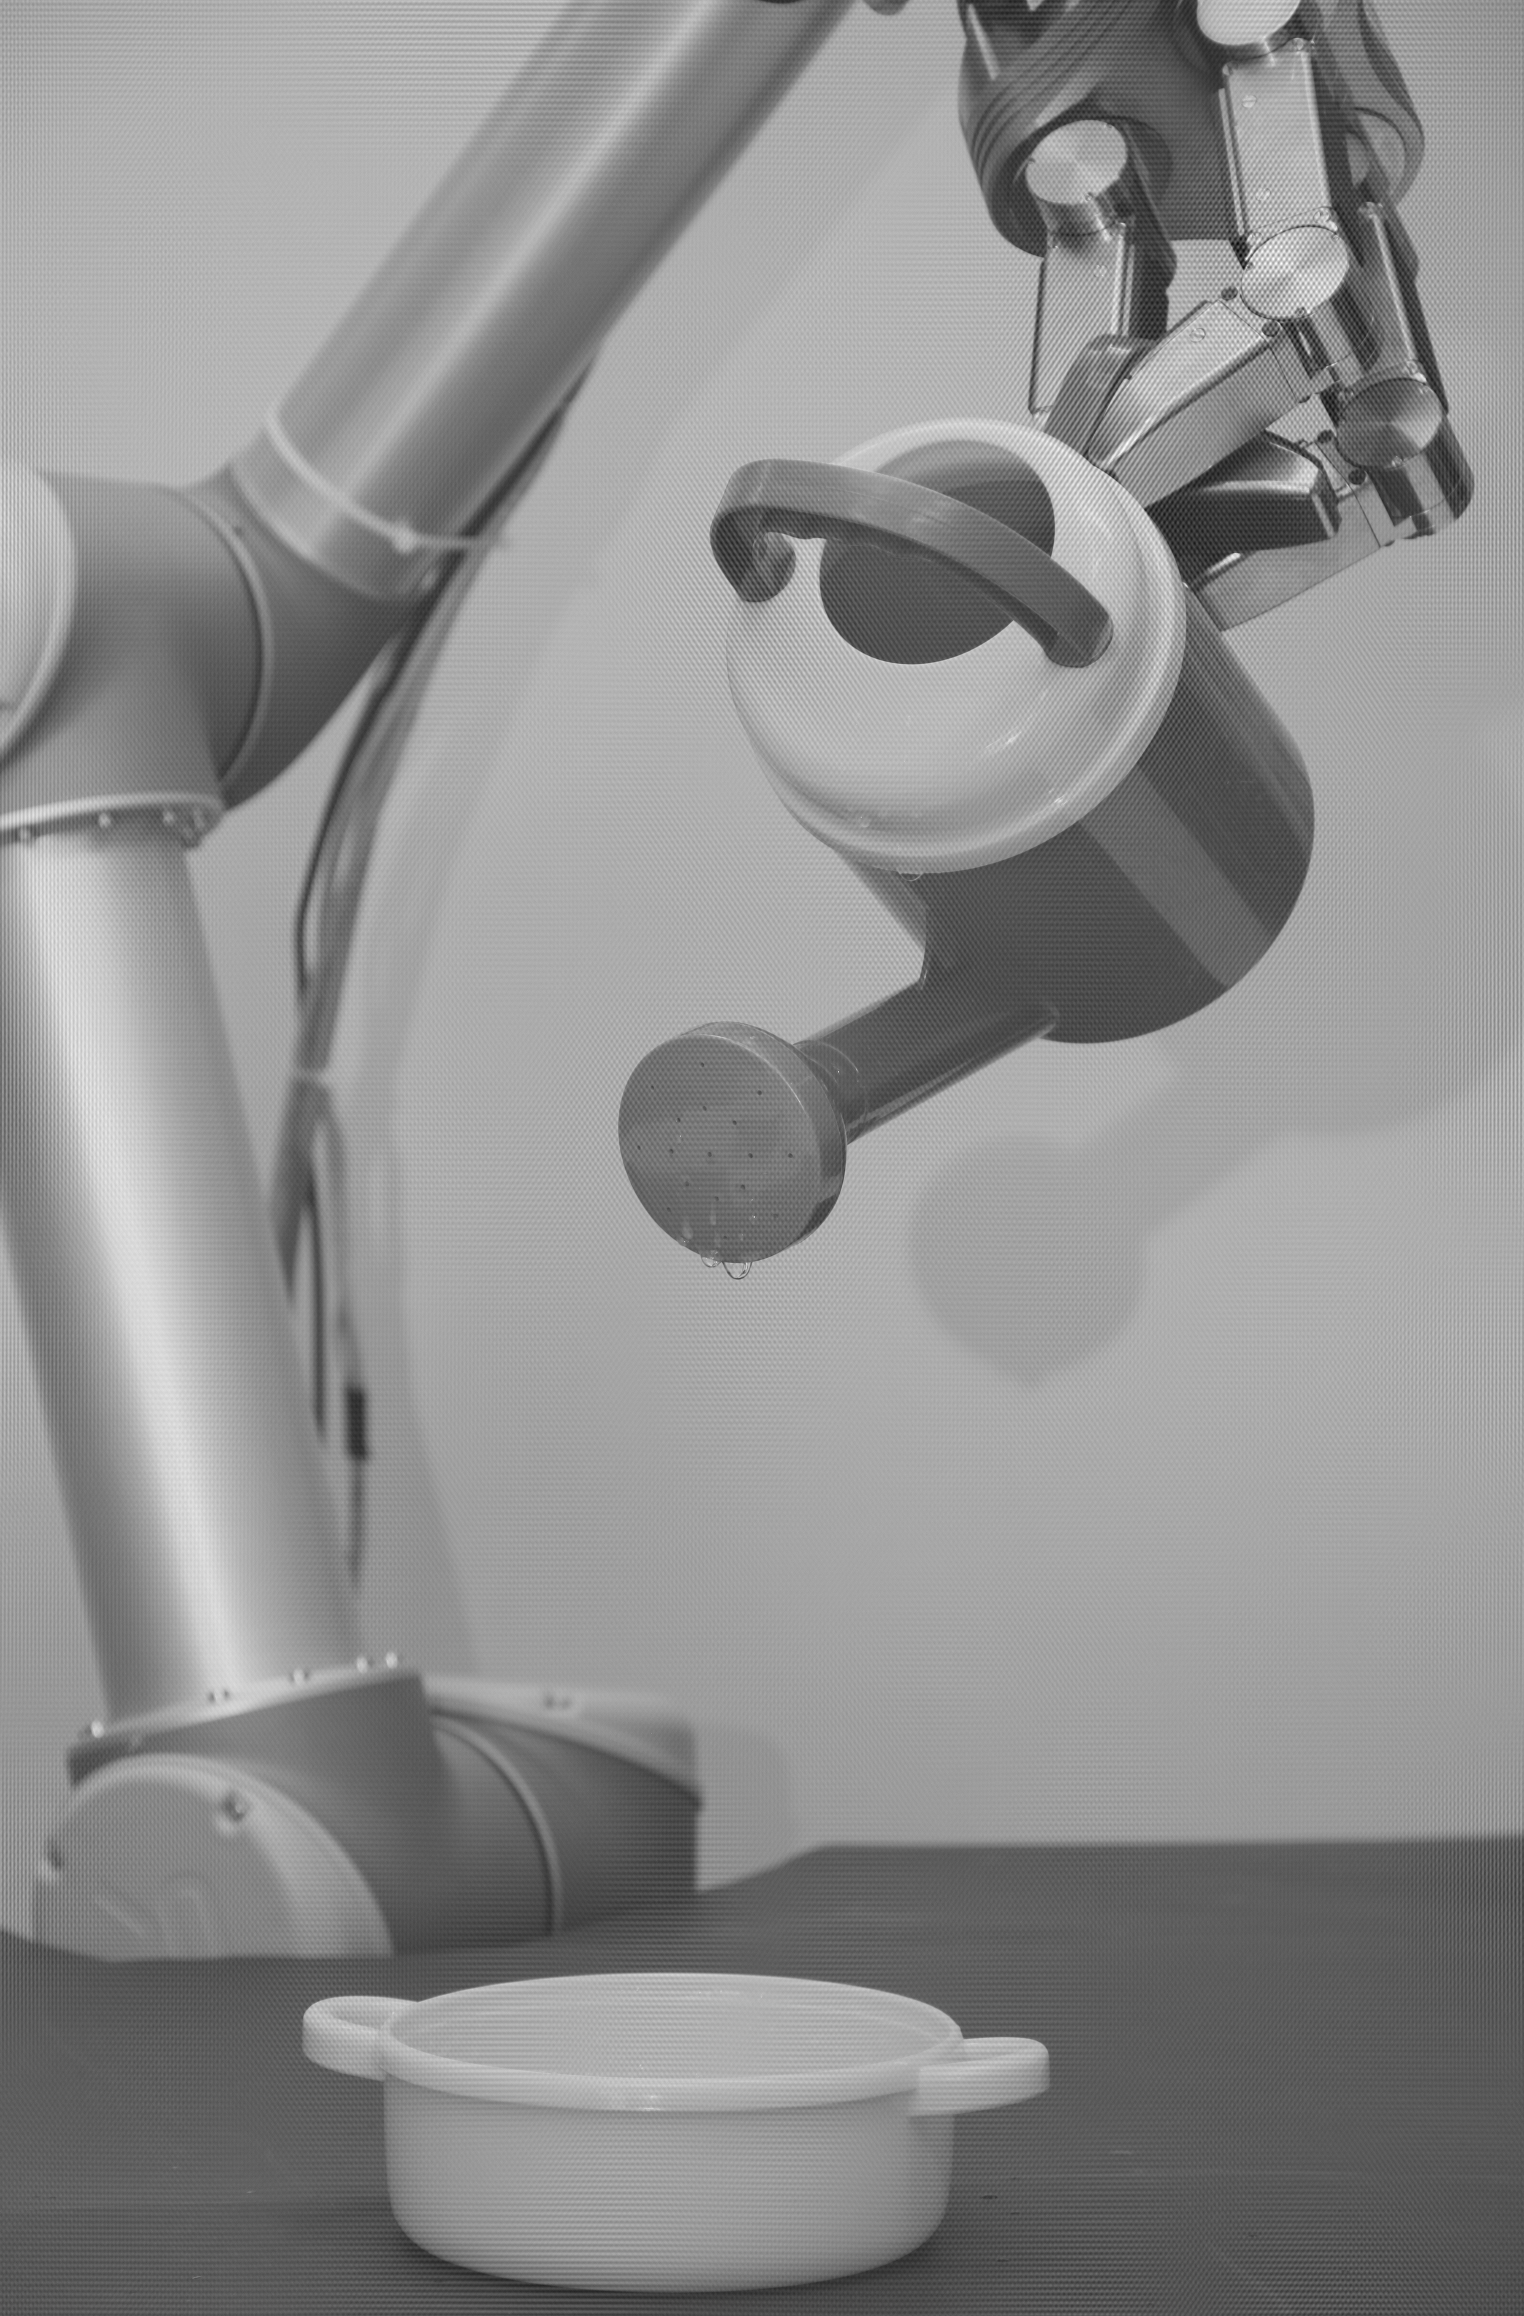
\includegraphics[width=\textwidth]{img4/Image4_2.png}
        \caption{Image4\_2 with \\no restoration}
        \label{fig:img42_src}
    \end{subfigure}
    \begin{subfigure}[b]{0.23\textwidth}
        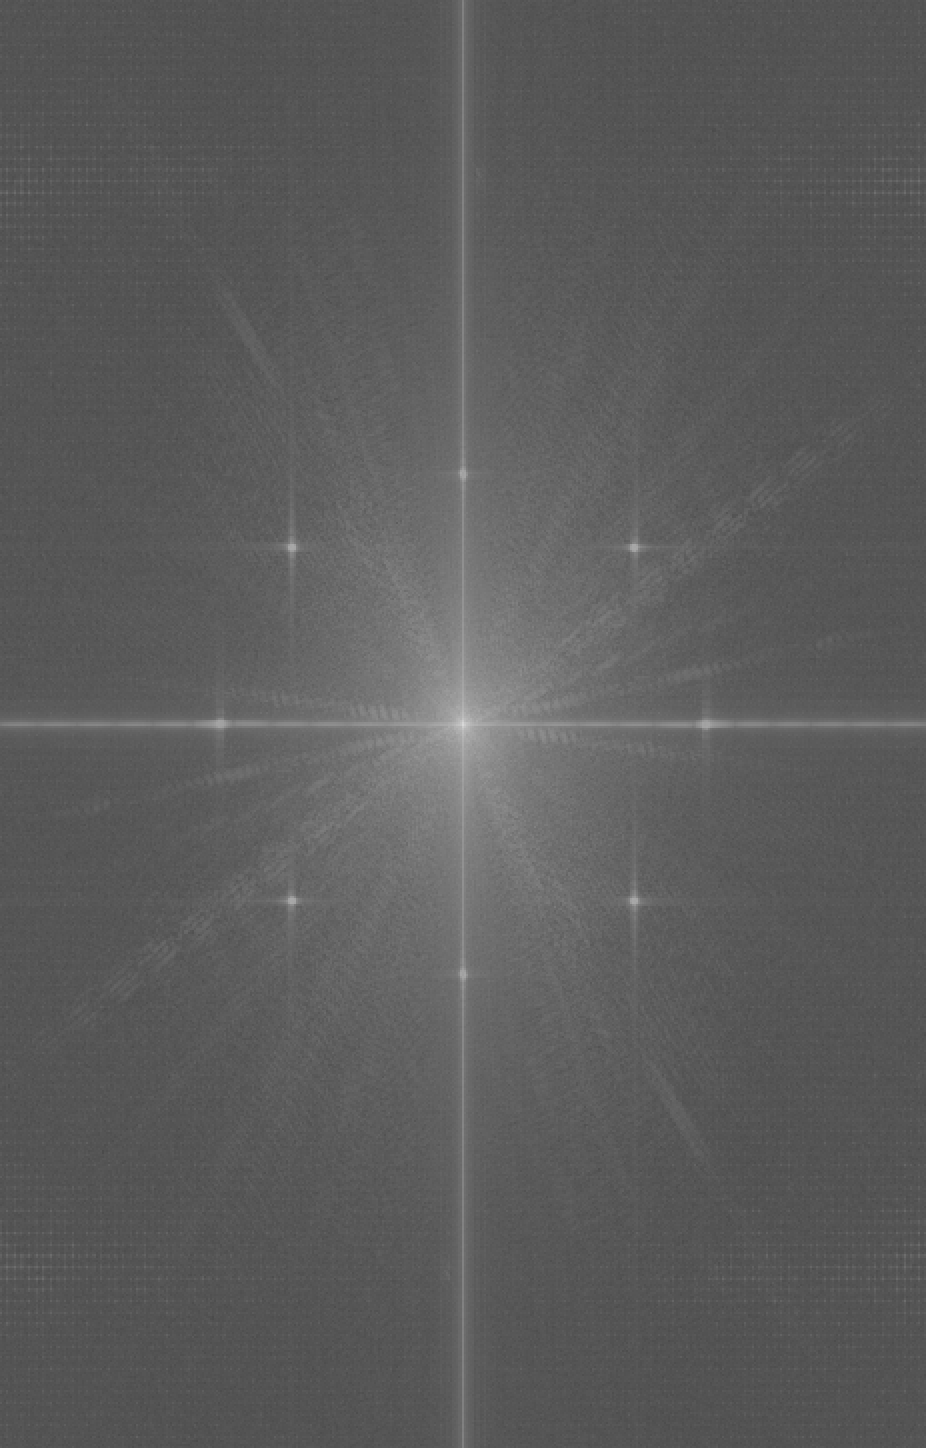
\includegraphics[width=\textwidth]{img4/Image4_2_freq_spec.png}
        \caption{Frequency spectrum of Image4\_2}
        \label{fig:img1_hist}
    \end{subfigure}
    \caption{Analysis of image 1}\label{fig:img1}
\end{figure}

